
\chapter{Listas}

\label{cap:listas} \index{lista} \index{elemento} \index{secuencia}

Una \textbf{lista} es un conjunto ordenado de valores que se identifican
por medio de un índice. Los valores que componen una lista se denominan
\textbf{elementos}. Las listas son similares a las cadenas, que son
conjuntos ordenados de caracteres, pero son mas generales, ya que
pueden tener elementos de cualquier tipo de dato. Las listas y las
cadenas—y otras conjuntos ordenados que veremos— se denominan \textbf{secuencias}.

\section{Creación de listas}

Hay varias formas de crear una nueva lista; la más simple es encerrar
los elementos entre corchetes (\verb+[+ y \verb+]+):\inputencoding{latin9}
\begin{lstlisting}
[10, 20, 30, 40]
["correo", "lapiz", "carro"]
\end{lstlisting}
\inputencoding{utf8}
El primer ejemplo es una lista de cuatro enteros, la segunda, una
lista de tres cadenas. Los elementos de una lista no tienen que tener
el mismo tipo. La siguiente lista contiene una cadena, un flotante,
un entero y (mirabile dictu) otra lista:\inputencoding{latin9}
\begin{lstlisting}
["hola", 2.0, 5, [10, 20]]
\end{lstlisting}
\inputencoding{utf8}
Cuando una lista está contenida por otra se dice que está \textbf{anidada}.

\index{lista!anidada}

Las listas que contienen enteros consecutivos son muy comunes, así
que Python proporciona una forma de crearlas:\inputencoding{latin9}
\begin{lstlisting}
>>> list(range(1,5))
[1, 2, 3, 4]
\end{lstlisting}
\inputencoding{utf8}
La función \texttt{range} toma dos argumentos y retorna una colección
que contiene todos los enteros desde el primero hasta el segundo,
¡incluyendo el primero y no el último! Esta colección se puede convertir
a lista con la función  \texttt{ list }

Hay otras formas de usar a \texttt{range}. Con un solo argumento crea
una lista que empieza en 0:\inputencoding{latin9}
\begin{lstlisting}
>>> list(range(10))
[0, 1, 2, 3, 4, 5, 6, 7, 8, 9]
\end{lstlisting}
\inputencoding{utf8}
Si hay un tercer argumento, este especifica el espacio entre los valores
sucesivos, que se denomina el \textbf{tamaño del paso}. Este ejemplo
cuenta de 1 a 10 con un paso de tamaño 2:\inputencoding{latin9}
\begin{lstlisting}
>>> list(range(1, 10, 2))
[1, 3, 5, 7, 9]
\end{lstlisting}
\inputencoding{utf8}
Finalmente, existe una lista especial que no contiene elementos. Se
denomina lista vacía, y se denota con \texttt{{[}{]}}.

Con todas estas formas de crear listas sería decepcionante si no pudiéramos
asignar listas a variables o pasarlas como parámetros a funciones.
De hecho, podemos hacerlo:\inputencoding{latin9}
\begin{lstlisting}
>>> vocabulario = ["mejorar", "castigar", "derrocar"]
>>> numeros = [17, 123]
>>> vacia = []
>>> print(vocabulario, numeros, vacia)
["mejorar", "castigar", "derrocar"] [17, 123] []
\end{lstlisting}
\inputencoding{utf8}
\section{Accediendo a los elementos}

\index{lista!elemento} \index{acceso}

La sintaxis para acceder a los elementos de una lista es la misma
que usamos en las cadenas—el operador corchete (\texttt{{[}{]}}).
La expresión dentro de los corchetes especifica el índice. Recuerde
que los índices o posiciones empiezan desde 0:\inputencoding{latin9}
\begin{lstlisting}
print(numeros[0])
numeros[1] = 5
\end{lstlisting}
\inputencoding{utf8}
El operador corchete para listas puede aparecer en cualquier lugar
de una expresión. Cuanto aparece al lado izquierdo de una asignación
cambia uno de los elementos de la lista de forma que el elemento 1
de \texttt{numeros}, que tenía el valor 123, ahora es 5.

Cualquier expresión entera puede usarse como índice:\inputencoding{latin9}
\begin{lstlisting}
>>> numeros[3-2]
5
>>> numeros[1.0]
TypeError: sequence index must be integer
\end{lstlisting}
\inputencoding{utf8}
Si usted intenta leer o escribir un elemento que no existe, obtiene
un error en tiempo de ejecución:

\index{error en tiempo de ejecución}\inputencoding{latin9}
\begin{lstlisting}
>>> numeros[2] = 5
IndexError: list assignment index out of range
\end{lstlisting}
\inputencoding{utf8}
Si el índice tiene un valor negativo, cuenta hacia atrás desde el
final de la lista:\inputencoding{latin9}
\begin{lstlisting}
>>> numeros[-1]
5
>>> numeros[-2]
17
>>> numeros[-3]
IndexError: list index out of range
\end{lstlisting}
\inputencoding{utf8}
\texttt{numeros{[}-1{]}} es el último elemento de la lista, \texttt{numeros{[}-2{]}}
es el penúltimo, y \texttt{numeros{[}-3{]}} no existe.

Usualmente se usan variables de ciclo como índices de listas:\inputencoding{latin9}
\begin{lstlisting}
combatientes = ["guerra", "hambruna", "peste", "muerte"]

i = 0
while i < 4:
  print(combatientes[i])
  i = i + 1
\end{lstlisting}
\inputencoding{utf8}
Este ciclo \texttt{while} cuenta de 0 a 4. Cuando la variable de ciclo
\texttt{i} es 4, la condición falla y el ciclo termina. El cuerpo
del ciclo se ejecuta solamente cuando \texttt{i} es 0, 1, 2, y 3.

En cada iteración del ciclo, la variable \texttt{i} se usa como un
índice a la lista, imprimiendo el \texttt{i}-ésimo elemento. Este
patrón se denomina \textbf{recorrido de una lista}.

\index{lista!recorrido de una} \index{recorrido!lista}

\section{Longitud de una lista}

\index{longitud} \index{lista!longitud}

La función \texttt{len} retorna la longitud de una lista. Es una buena
idea usar este valor como límite superior de un ciclo en vez de una
constante. De ésta forma, si la lista cambia, usted no tendrá que
cambiar todos los ciclos del programa, ellos funcionarán correctamente
para listas de cualquier tamaño:\inputencoding{latin9}
\begin{lstlisting}
combatientes = ["guerra", "hambruna", "peste", "muerte"]

i = 0
while i < len(combatientes):
  print(combatientes[i])
  i = i + 1
\end{lstlisting}
\inputencoding{utf8}
La última vez que el ciclo se ejecuta \texttt{i} es \texttt{len(combatientes)
- 1}, que es la posición del último elemento. Cuando \texttt{i} es
igual a \texttt{len(combatientes)}, la condición falla y el cuerpo
no se ejecuta, lo que está muy bien , ya que \texttt{len(combatientes)}
no es un índice válido.

Aunque una lista puede contener a otra, la lista anidada se sigue
viendo como un elemento único. La longitud de esta lista es cuatro:\inputencoding{latin9}
\begin{lstlisting}
['basura!', 1, ['Brie', 'Roquefort', 'Pol le Veq'], 
 [1, 2, 3]]
\end{lstlisting}
\inputencoding{utf8}
\section{Pertenencia}

\index{lista!pertenencia} \index{operador in} \index{operador!in}

\texttt{in} es un operador booleano que chequea la pertenencia de
un valor a una secuencia. Lo usamos en la Sección~\ref{in} con cadenas,
pero también funciona con listas y otras secuencias:\inputencoding{latin9}
\begin{lstlisting}
>>> combatientes = ["guerra", "hambruna", "peste", "muerte"]
>>> 'peste' in combatientes
True
>>> 'corrupcion' in combatientes
False
\end{lstlisting}
\inputencoding{utf8}
Ya que ``peste'' es un miembro de la lista \texttt{combatientes},
el operador \texttt{in} retorna cierto. Como ``corrupcion'' no está
en la lista, \texttt{in} retorna falso.

Podemos usar el operador lógico \texttt{not} en combinación con el
\texttt{in} para chequear si un elemento no es miembro de una lista:\inputencoding{latin9}
\begin{lstlisting}
>>> 'corrupcion' not in combatientes
True
\end{lstlisting}
\inputencoding{utf8}
\section{Listas y ciclos \texttt{for}}

\index{ciclo for} \index{lista!ciclo for} \index{recorrido}

El ciclo \texttt{for} que vimos en la Sección~\ref{for} también
funciona con listas. La sintaxis generalizada de un ciclo \texttt{for}
es:\inputencoding{latin9}
\begin{lstlisting}
for VARIABLE in LISTA:
  CUERPO
\end{lstlisting}
\inputencoding{utf8}
Esto es equivalente a:\inputencoding{latin9}
\begin{lstlisting}
i = 0
while i < len(LISTA):
  VARIABLE = LISTA[i]
  CUERPO
  i = i + 1
\end{lstlisting}
\inputencoding{utf8}
El ciclo \texttt{for} es más conciso porque podemos eliminar la variable
de ciclo \texttt{i}. Aquí está el ciclo de la sección anterior escrito
con un \texttt{for} en vez de un while: \inputencoding{latin9}
\begin{lstlisting}
for combatiente in combatientes:
  print(combatiente)
\end{lstlisting}
\inputencoding{utf8}
Casi se lee como en español: ``Para (cada) combatiente en (la lista
de) combatientes, imprima (el nombre del) combatiente''.

Cualquier expresión que cree una lista puede usarse en un ciclo \texttt{for}:\inputencoding{latin9}
\begin{lstlisting}
for numero in range(20):
  if numero % 2 == 0:
    print(numero)

for fruta in ["banano", "manzana", "pera"]:
  print("Me gustaria comer " + fruta + "s!")
\end{lstlisting}
\inputencoding{utf8}
El primer ejemplo imprime todos los números pares entre uno y diecinueve.
El segundo expresa entusiasmo sobre varias frutas.

\section{Operaciones sobre listas}

\index{operaciones sobre listas} \index{operación!sobre listas}

El operador \texttt{+} concatena listas:

\index{concatenación!de listas}\inputencoding{latin9}
\begin{lstlisting}
>>> a = [1, 2, 3]
>>> b = [4, 5, 6]
>>> c = a + b
>>> print(c)
[1, 2, 3, 4, 5, 6]
\end{lstlisting}
\inputencoding{utf8}
Similarmente, el operador \texttt{{*}} repite una lista un número
de veces determinado:

\index{repetición!de listas}\inputencoding{latin9}
\begin{lstlisting}
>>> [0] * 4
[0, 0, 0, 0]
>>> [1, 2, 3] * 3
[1, 2, 3, 1, 2, 3, 1, 2, 3]
\end{lstlisting}
\inputencoding{utf8}
El primer ejemplo repite \texttt{{[}0{]}} cuatro veces. El segundo
repite \texttt{{[}1, 2, 3{]}} tres veces.

\section{Segmentos de listas}

\index{segmento} \index{lista!segmento}

Las operaciones para sacar segmentos de cadenas que vimos en la Sección~\ref{slice}
también funcionan con listas:\inputencoding{latin9}
\begin{lstlisting}
>>> lista = ['a', 'b', 'c', 'd', 'e', 'f']
>>> lista[1:3]
['b', 'c']
>>> lista[:4]
['a', 'b', 'c', 'd']
>>> lista[3:]
['d', 'e', 'f']
>>> lista[:]
['a', 'b', 'c', 'd', 'e', 'f']
\end{lstlisting}
\inputencoding{utf8}
\section{Las listas son mutables}

\index{mutable!lista} \index{lista!mutable}

Las listas son mutables y no tienen la restricción de las cadenas,
esto quiere decir que podemos cambiar los elementos internos usando
el operador corchete al lado izquierdo de una asignación.\inputencoding{latin9}
\begin{lstlisting}
>>> fruta = ["banano", "manzana", "pera"]
>>> fruta[0] = "mandarina"
>>> fruta[-1] = "naranja"
>>> print(fruta)
['mandarina', 'manzana', 'naranja']
\end{lstlisting}
\inputencoding{utf8} Con el operador segmento podemos actualizar varios elementos a la
vez:\inputencoding{latin9}
\begin{lstlisting}
>>> lista = ['a', 'b', 'c', 'd', 'e', 'f']
>>> lista[1:3] = ['x', 'y']
>>> print(lista)
['a', 'x', 'y', 'd', 'e', 'f']
\end{lstlisting}
\inputencoding{utf8}
También podemos eliminar varios elementos asignándoles la lista vacía:\inputencoding{latin9}
\begin{lstlisting}
>>> lista = ['a', 'b', 'c', 'd', 'e', 'f']
>>> lista[1:3] = []
>>> print(lista)
['a', 'd', 'e', 'f']
\end{lstlisting}
\inputencoding{utf8}
Igualmente, podemos agregar elementos a una lista apretándolos dentro
de un segmento vacío en la posición que deseamos:\inputencoding{latin9}
\begin{lstlisting}
>>> lista = ['a', 'd', 'f']
>>> lista[1:1] = ['b', 'c']
>>> print(lista)
['a', 'b', 'c', 'd', 'f']
>>> lista[4:4] = ['e']
>>> print(lista)
['a', 'b', 'c', 'd', 'e', 'f']
\end{lstlisting}
\inputencoding{utf8}
\section{Otras operaciones sobre listas}

\index{operación sobre listas}

Usar segmentos para insertar y borrar elementos de una lista es extraño
y propenso a errores. Hay mecanismos alternativos más legibles como
\texttt{del} que elimina un elemento de una lista.

\index{borrado!en listas} \index{borrado en listas} \index{del}\inputencoding{latin9}
\begin{lstlisting}
>>> a = ['one', 'two', 'three']
>>> del a[1]
>>> a
['one', 'three']
\end{lstlisting}
\inputencoding{utf8}
Como es de esperar, \texttt{del} recibe índices negativos, y causa
errores en tiempo de ejecución si el índice está fuera de rango.

También se puede usar un segmento como argumento a \texttt{del}:\inputencoding{latin9}
\begin{lstlisting}
>>> lista = ['a', 'b', 'c', 'd', 'e', 'f']
>>> del lista[1:5]
>>> print(lista)
['a', 'f']
\end{lstlisting}
\inputencoding{utf8}
Como de costumbre, los segmentos seleccionan todos los elementos hasta
el segundo índice, sin incluirlo.

La función \texttt{append} agrega un elemento (o una lista) al final
de una lista existente:\inputencoding{latin9}
\begin{lstlisting}
>>> a = ['uno', 'dos']
>>> a.append('tres')
>>> print(a)
\end{lstlisting}
\inputencoding{utf8}
Observe que se llama con la notación punto, a diferencia de \texttt{len}
y \texttt{del}.

\section{Objetos y valores}

\index{objeto} \index{valor}

Si ejecutamos estas asignaciones\inputencoding{latin9}
\begin{lstlisting}
a = "banana"
b = "banana"
\end{lstlisting}
\inputencoding{utf8}
sabemos que \texttt{a} y \texttt{b} se referirán a una cadena con
las letras \texttt{``banana''}. Pero no podemos afirmar que sea
la {\em misma} cadena.

Hay dos situaciones posibles:

\beforefig \centerline{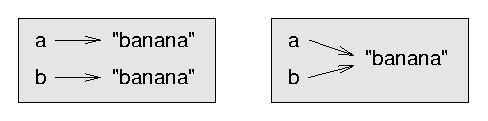
\includegraphics{illustrations/list1}}
\afterfig

En un caso, \texttt{a} y \texttt{b} se refieren a cosas distintas
que tienen el mismo valor. En el segundo caso, se refieren a la misma
cosa. Estas ``cosas'' tienen nombres—se denominan \textbf{objetos}.
Un objeto es algo a lo que se puede referir una variable.

Cada objeto tiene un \textbf{identificador} único, que podemos obtener
con la función \texttt{id}. Imprimiendo el identificador de \texttt{a}
y \texttt{b}, podemos saber si se refieren al mismo objeto.\inputencoding{latin9}
\begin{lstlisting}
>>> id(a)
135044008
>>> id(b)
135044008
\end{lstlisting}
\inputencoding{utf8}
De hecho, obtenemos el mismo identificador dos veces, lo que nos dice
que Python sólo creó una cadena, y que \texttt{a} y \texttt{b} se
refieren a ella.

Las listas, por otro lado, se comportan de manera diferente. Cuando
creamos dos listas obtenemos dos objetos:\inputencoding{latin9}
\begin{lstlisting}
>>> a = [1, 2, 3]
>>> b = [1, 2, 3]
>>> id(a)
135045528
>>> id(b)
135041704
\end{lstlisting}
\inputencoding{utf8}
Así que el diagrama de estados luce así:

\beforefig \centerline{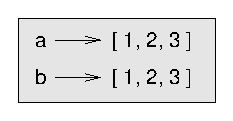
\includegraphics{illustrations/list2}}
\afterfig

\texttt{a} y \texttt{b} tienen el mismo valor pero no se refieren
al mismo objeto.

\section{Alias}

\index{alias} \index{referencia!alias}

Como las variables se pueden referir a objetos, si asignamos una variable
a otra, las dos se referirán al mismo objeto:\inputencoding{latin9}
\begin{lstlisting}
>>> a = [1, 2, 3]
>>> b = a
\end{lstlisting}
\inputencoding{utf8}
En este caso el diagrama de estados luce así:

\beforefig \centerline{
\includegraphics{illustrations/list3}}
\afterfig

Como la misma lista tiene dos nombres distintos, \texttt{a} y \texttt{b},
podemos decir que b es un \textbf{alias} de a. Los cambios que se
hagan a través de un alias afectan al otro:\inputencoding{latin9}
\begin{lstlisting}
>>> b[0] = 5
>>> print(a)
[5, 2, 3]
\end{lstlisting}
\inputencoding{utf8}
Aunque este comportamiento puede ser útil, algunas veces puede ser
indeseable. En general, es más seguro evitar los alias cuando se está
trabajando con objetos mutables. Para objetos inmutables no hay problema.
Esta es la razón por la que Python tiene la libertad de crear alias
a cadenas cuando ve la oportunidad de economizar memoria. Pero tenga
en cuenta que esto puede variar en las diferentes versiones de Python;
por lo tanto no es recomendable realizar programas que dependan de
este comportamiento.

\section{Clonando listas}

\index{lista!clonando} \index{clonando}

Si queremos modificar una lista y conservar una copia de la original,
necesitamos realizar una copia de la lista, no sólo de la referencia.
Este proceso se denomina \textbf{clonación}, para evitar la ambigüedad
de la palabra ``copiar''.

La forma más sencilla de clonar una lista es usar el operador segmento:\inputencoding{latin9}
\begin{lstlisting}
>>> a = [1, 2, 3]
>>> b = a[:]
>>> print(b)
[1, 2, 3]
\end{lstlisting}
\inputencoding{utf8}
Al tomar cualquier segmento de \texttt{a} creamos una nueva lista.
En este caso el segmento comprende toda la lista.

Ahora podemos realizar cambios a \texttt{b} sin preocuparnos por \texttt{a}:\inputencoding{latin9}
\begin{lstlisting}
>>> b[0] = 5
>>> print(a)
[1, 2, 3]
\end{lstlisting}
\inputencoding{utf8}
¿Como sería un diagrama de estados para \texttt{a} y \texttt{b} antes
y después de este cambio? 

\section{Listas como parámetros}

\index{listas!como parámetros} \index{parámetro} \index{parámetro!lista}

Pasar una lista como argumento es pasar un alias (o una referencia),
no una copia de ella. Por ejemplo, la función \texttt{cabeza} toma
una lista como parámetro y retorna el primer elemento:\inputencoding{latin9}
\begin{lstlisting}
def cabeza(lista):
  return lista[0]
\end{lstlisting}
\inputencoding{utf8}
Se puede usar así:\inputencoding{latin9}
\begin{lstlisting}
>>> numeros = [1, 2, 3]
>>> cabeza(numeros)
1
\end{lstlisting}
\inputencoding{utf8}
El parámetro \texttt{lista} y la variable \texttt{numeros} son alias
para el mismo objeto. El diagrama de estados luce así:

\beforefig \centerline{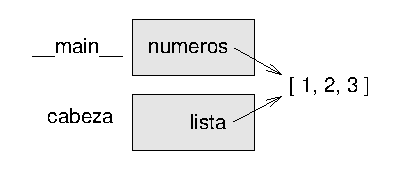
\includegraphics{illustrations/stack5}}
\afterfig

Como el objeto lista está compartido por dos marcos, lo dibujamos
en el medio.

Si una función modifica un parámetro de tipo lista, el que hizo el
llamado ve los cambios. Por ejemplo, \texttt{borrarCabeza} borra el
primer elemento de una lista:\inputencoding{latin9}
\begin{lstlisting}
def borrarCabeza(lista):
  del lista[0]
\end{lstlisting}
\inputencoding{utf8}
Y se puede usar así::\inputencoding{latin9}
\begin{lstlisting}
>>> numeros = [1, 2, 3]
>>> borrarCabeza(numeros)
>>> print(numeros)
[2, 3]
\end{lstlisting}
\inputencoding{utf8}
Si una función retorna una lista, retorna una referencia a ella. Por
ejemplo, la función \texttt{cola} retorna una lista que contiene todos
los elementos, excepto el primero:\inputencoding{latin9}
\begin{lstlisting}
def cola(lista):
  return lista[1:]
\end{lstlisting}
\inputencoding{utf8}
\texttt{cola} se puede usar así:\inputencoding{latin9}
\begin{lstlisting}
>>> numeros = [1, 2, 3]
>>> resto = cola(numeros)
>>> print(resto)
[2, 3]
\end{lstlisting}
\inputencoding{utf8}
Como el valor de retorno se creó con el operador segmento, es una
nueva lista. La creación de \texttt{resto}, y los cambios subsecuentes
sobre esta variable no tienen efecto sobre \texttt{numeros}.

\section{Listas anidadas}

\label{nested lists} \index{listas anidadas} \index{lista!anidada}

Una lista anidada aparece como elemento dentro de otra lista. En la
siguiente lista, el tercer elemento es una lista anidada:\inputencoding{latin9}
\begin{lstlisting}
>>> lista = ["hola", 2.0, 5, [10, 20]]
\end{lstlisting}
\inputencoding{utf8}
Si imprimimos \texttt{lista{[}3{]}}, vemos \texttt{{[}10, 20{]}}.
Para tomar un elemento de la lista anidada podemos realizar dos pasos:\inputencoding{latin9}
\begin{lstlisting}
>>> elt = lista[3]
>>> elt[0]
10
\end{lstlisting}
\inputencoding{utf8} O, los podemos combinar:\inputencoding{latin9}
\begin{lstlisting}
>>> lista[3][1]
20
\end{lstlisting}
\inputencoding{utf8}
Las aplicaciones del operador corchete se evalúan de izquierda a derecha,
así que ésta expresión obtiene el elemento 3 de \texttt{lista} y extrae
de allí el elemento 1.

\section{Matrices}

\index{matriz} \index{lista!anidada}

Las listas anidadas se usan a menudo para representar matrices. Por
ejemplo, la matriz:

\beforefig \centerline{
\includegraphics{illustrations/matrix}}
\afterfig

se puede representar así:\inputencoding{latin9}
\begin{lstlisting}
>>> matriz = [[1, 2, 3], [4, 5, 6], [7, 8, 9]]
\end{lstlisting}
\inputencoding{utf8}
\texttt{matriz} es una lista con tres elementos, cada uno es una fila.
Podemos seleccionar una fila de la manera usual:\inputencoding{latin9}
\begin{lstlisting}
>>> matriz[1]
[4, 5, 6]
\end{lstlisting}
\inputencoding{utf8}
O podemos extraer un elemento individual de la matriz usando dos índices:\inputencoding{latin9}
\begin{lstlisting}
>>> matriz[1][1]
5
\end{lstlisting}
\inputencoding{utf8}
El primero escoge la fila, y el segundo selecciona la columna. Aunque
esta forma de representar matrices es común, no es la única posibilidad.
Una pequeña variación consiste en usar una lista de columnas en lugar
de una lista de filas. Más adelante veremos una alternativa más radical,
usando un diccionario.

\index{diccionario} \index{fila} \index{columna}

\section{Cadenas y listas}

\index{función split} \index{función join}

Dos de las funciones más usadas de las cadenas implican listas de
cadenas. \texttt{split} separa una cadena en una lista de palabras.
Por defecto, cualquier número de espacios en blanco sirven como criterio
de separación:
\begin{verbatim}
>>> cancion = "La vida es un ratico..."
>>> str.split(cancion)
['La', 'vida', 'es', 'un', 'ratico...']
\end{verbatim}
Un argumento opcional denominado \textbf{delimitador} se puede usar
para especificar que caracteres usar como criterio de separación.
El siguiente ejemplo usa la cadena \texttt{an} como delimitador:\inputencoding{latin9}
\begin{lstlisting}
>>> str.split( "La rana que canta", "an")
['La r', 'a que c', 'ta']
\end{lstlisting}
\inputencoding{utf8}
Note que el delimitador no aparece en la lista resultante.

La función \texttt{join} es la inversa de \texttt{split}. Toma una
lista de cadenas y las concatena usando como separador a la cadena
que la llama con notación punto:\inputencoding{latin9}
\begin{lstlisting}
>>> m = ['La', 'vida', 'es', 'un', 'ratico']
>>> " ".join(m)
'La vida es un ratico'
\end{lstlisting}
\inputencoding{utf8}
Si usamos una cadena diferente de espacio, obtenemos otro resultado:\inputencoding{latin9}
\begin{lstlisting}
>>> "_".join(m)
'La_vida_es_un_ratico'
\end{lstlisting}
\inputencoding{utf8}
\section{Glosario}
\begin{description}
\item [{Lista:}] colección de objetos que recibe un nombre. Cada objeto
se identifica con un índice o número entero positivo.
\item [{Índice:}] valor o variable entero que indica la posición de un
elemento en una lista.
\item [{Elemento:}] uno de los valores dentro de una lista (u otra secuencia).
El operador corchete selecciona elementos de una lista.
\item [{Secuencia:}] los tipos de datos que contienen un conjunto ordenado
de elementos, identificados por índices.
\item [{Lista anidada:}] lista que es elemento de otra lista.
\item [{Recorrido de una lista:}] es el acceso secuencial de cada elemento
de una lista.
\item [{Objeto:}] una cosa a la que una variable se puede referir.
\item [{Alias:}] cuando varias variables tienen referencias hacia el mismo
objeto.
\item [{Clonar:}] crear un objeto con el mismo valor que un objeto preexistente.
Copiar una referencia a un objeto crea un alias, pero no clona el
objeto.
\item [{Delimitador:}] carácter o cadena que se usa para indicar el lugar
donde una cadena debe ser separada.

\index{lista} \index{índice} \index{secuencia} \index{elemento}
\index{lista anidada} \index{recorrido de una lista} \index{objeto}
\index{alias} \index{clonar} \index{delimitador}
\end{description}

\section{Ejercicios}

Para cada función, agregue chequeo de tipos y pruebas unitarias.
\begin{enumerate}
\item Escriba una función llamada medio que reciba una lista y retorne una
nueva lista que contenga todos los elementos de la lista de entrada
excepto el primero y el último. Por ejemplo, medio({[}1,2,3,4{]})
debe retornar {[}2,3{]}.
\item Escriba una función llamada cortar que reciba una lista y la modifique
eliminando el primer y el último elemento, retornando None.
\item Escriba una función que recorra una lista de cadenas imprimiendo la
longitud de cada una. ¿Qué pasa si usted le pasa un entero a \texttt{len}?
\item Describa la relación entre las expresiones:

\texttt{cadena} \hfill{}\texttt{' '.join(str.split(cadena))}

¿Son iguales para todas las cadenas?

¿Cuando serían diferentes?
\item Escriba una función llamada \verb+esta_ordenada+ que tome una lista
como parámetro y retorne True si la lista está ordenada de forma ascendente
o False si no lo está. Usted puede asumir como precondición que los
elementos son comparables con los operadores relacionales. Por ejemplo:

\verb+esta_ordenada([1,2,2])+ debe retornar True

\verb+esta_ordenada(['b','a'])+ debe retornar False.
\item Dos palabras son anagramas si se pueden reordenar las letras de una
palabra para formar la otra. Escriba una función llamada \verb+es_anagrama+
que tome dos cadenas y retorne True si son anagramas y False en caso
contrario.
\item Escriba una función llamada \verb+eliminar_duplicados+ que reciba
una lista y retorne una nueva lista con los elementos únicos de la
original. No necesitan estar en el mismo orden.
\item Escriba dos versiones de una función que lea el archivo palabras.txt
y construya una lista con un elemento por palabra. Una versión usará
el método append y la otra la construcción t=t+{[}x{]}. ¿Cual es mas
lenta? ¿Por qué? Pista: use el módulo time para medir lo que tarda
la ejecución de las versiones.

palabras.txt: \url{https://github.com/abecerra/thinkcs-py_es/releases/download/thinkcs-py_es_e2-rc1/palabras.txt}

Solución: \url{http://thinkpython.com/code/wordlist.py}
\item Si hay un grupo de 23 personas, ¿cual es la probabilidad de que dos
tengan la misma fecha de nacimiento?. Este valor puede estimarse generando
muestras aleatorias de 23 cumpleaños y contando las coincidencias.
Pista: consulte la función randint del módulo random.

Solución: \url{http://thinkpython.com/code/birthday.py}
\item Dos palabras son un ``par inverso'' si cada una es la inversa de
la otra. Escriba un programa que encuentre todos los pares inversos
del español (palabras.txt).

Solución: \url{http://thinkpython.com/code/reverse_pair.py}
\item Dos palabras se entretejen si tomando las letras de las dos, alternándose,
se puede formar una nueva palabra. Por ejemplo: 'pie' y 'en' se entretejen
en 'peine'.

Solución: \url{http://thinkpython.com/code/interlock.py} 
\end{enumerate}

